\documentclass[12pt]{article}

\usepackage[utf8]{inputenc}


\usepackage{caption}
\usepackage{amsmath}
\usepackage{graphicx}
\usepackage{amssymb}
\usepackage{float}
\usepackage{multirow}
\usepackage{setspace} \setstretch{0.9}
% set font size to 11pt


\setlength{\parskip}{\baselineskip}%
\setlength{\parindent}{0pt}%


\begin{document}

\title{Wave Transmission}
\author{lwp26}
\date{Feburary 2023}
\maketitle

\begin{abstract}
    \centering
    This report investigates properties of standing waves produced by the reflection of microwaves under different boundary conditions.
    The wavelength and phase velocity of standing waves are measured by observing the positions of minima in a slotted line.
    The phase shift is observed to change $\pi$ as the interference changes from destructive to constructive.
    The amplitude reflection coefficient for a brass screw is also calculated from the change in maximum amplitudes.
    The refractive index of perspex, glass and teflon is measured for microwaves. Inconsistencies in refractive indicies obtained for 
    same materials is discussed and thought to be because of interference caused by uneven air gap between the strip line and the material.
    The resonant frequency of a resonator setup of the strip line is found and a plot of the response is produced.

\end{abstract}


\section{Introduction}

\subsection{Background}

Waves are a fundamental part of physics with many different applications,
in the efficient transmission of information and energy. 
In this report, we will be looking at the transmission of waves through a medium, 
and how the transmission of waves can be affected by the medium.


\subsection{Aims}
\begin{itemize}
    \item To create and observe the effect of combining waves travelling in opposite directions - 
    which produces standing waves.
    \item To measure the wavelength and velocity of microwaves in air by observing standing waves
    in a coaxial line.
    \item To measure the velocity of microwaves in some solid material (e.g. teflon, perspex and
    glass) from the change in travel time when the material is substituted for air, and to
    characterise the material by its refractive index, n.
    \item To build a microwave resonator, by making a section line with highly reflective ends. To
    plot and interpret the response versus frequency for resonators of two different lengths.
    \item To identify sources of error in the instruments and procedures used, and to suggest
    improvements.
\end{itemize}

\section{Method}

\subsection{Apparatus}

\begin{itemize}
    \item Computer controlled microwave source
    \item Slotted Line - A fine probe can be moved along the line to measure the amplitudes of the waves at different points. The end of the line can be fitted with a short or open circuit to include reflections. Loads can also be added using a strip line.
    \item Strip Line - allows different materials to be introduced into the wave field space between the suspended live conductor and the ground plane.
    \item Data logger - to record amplitude at specific distances along the slotted line
\end{itemize}

\subsection{Wavelength and Phase Velocity of Standing Waves}

The short circuit plug at the end of the slotted line is fitted to produce standing waves in the line. The probe is moved along the line to find two positions of minima. The average distance between the minima is found and the wavelength is calculated. The phase velocity is then calculated from the wavelength and the frequency of the microwave source.

\subsection{Amplitude Reflection Coefficient}

The closed circuit plug has a amplitude reflection coefficient $\rho = -1$, However the reflection coefficient of the open circuit plug is not known.
The open circuit plug is fitted to the end of the slotted line. The probe is moved along the line to find the new positions of minima to the right of the original minima.
The average distance between the minima is found and the wavelength is calculated. The fraction of average shift over the wavelength is then calculated. The expected value of the fraction is $\frac{1}{4}$.
The \textit{power} amplitudes of the constructive and destructive interference are measured at the two positions of minima and the \textit{standing wave ratio, $S$} can be calculated by using Eq 1.
The amplitude reflection coefficient is then calculated from $S$ using Eq 2.

\begin{equation}
    S^2 = \frac{A + B}{A - B}
    \label{eq:1}
\end{equation}
\begin{equation}
    \rho = \frac{S-1}{S+1}
    \label{eq:2}
\end{equation}

\subsection{Velocity of Microwaves in Different Materials}

The strip line is connected to the end of the slotted line to allow the microwaves to pass through.
A brass screw is used at the end of the strip line to reflect microwaves back into the slotted line.
The minima distance is measured before and after materials are introduced into the strip line.
The difference the minima is moved is also given by
\begin{equation}
    R - M = (n-1)d
    \label{eq:3}
\end{equation}

Where $n$ is the refractive index, $d$ is the length of the material along the strip line and $R$ and $M$ are the distances of minima on the slotted line.

Three materials were tested in the strip line, perspex, glass and teflon. The refractive indicies of these materials for visible light are $n = 1.49$, $n = 1.52$ and $n = 1.35$ respectively.
The lengths of the materials were $d = 30$ mm, $d = 60$ mm, $d = 90$ mm and $d = 120$ mm respectively.

\subsection{Transmission through a Resonator}

Two brass screws are now used at either end of the strip line. The screws are highly reflective, but not entirely.
The screws can produce a resonant standing wave in the strip line at a certain frequency called the \textit{resonant frequency}.
First a frequency sweep was done without the screws to observe the frequency response.
The screws were then fitted 120mm apart on the strip line and the frequency sweep was repeated.
The amplitude response was measured by the data logger and plotted against frequency.

\section{Results}

\begin{center}
    \captionof{table}{Measurements of wavelength and phase velocity of standing waves}
    \begin{tabular}{|c|c|c|c|c|c|}
    \hline
    Freq. & \multicolumn{2}{|c|}{Minima Positions $\pm0.5$} & N. Maximas &$\lambda\pm1.0$ & $u$ \\
    $f$/GHz & $P_1$/mm & $Q_1$/mm & $P_1$ to $Q_1$ & mm & mm/ns\\
    \hline 
    $2.399$	& $22$	& $523$	& $8$	& $125.25$	& $300.47\pm0.60$ \\
    $3.000$	& $59$	& $452$	& $8$	& $98.25$	& $294.75\pm0.75$ \\
    $3.600$	& $30$	& $488$	& $11$	& $83.27$	& $299.78\pm3.65$ \\
    \hline
    \end{tabular}
    \label{tab:1}
\end{center}

\begin{center}
    \captionof{table}{Amplitude reflection coefficients measured with slotted line}
    \begin{tabular}{|c|c|c|c|c|c|c|}
    \hline
    $f$ & $P_2$ & $(P_2-P_1)$ & $Q_2$ & $(Q_2-Q_1)$ & Average Shift & $\Delta / \lambda$ \\
    GHz & mm & mm & mm & mm & $\Delta$ mm & - \\
    \hline 
    $3.0$ & $33\pm0.5$ & $26\pm1.0$ & $431\pm0.5$ & $21\pm1.0$ & $23.5\pm2.0$ & $0.239\pm0.025$ \\
    \hline
    \end{tabular}
    \label{tab:2}
\end{center}

\begin{center}
    \captionof{table}{Amplitude reflection coefficients measured with slotted line}
    \begin{tabular}{|c|c|c|c|c|}
    \hline
    $(A+B)^2$ & $(A-B)^2$ & $S^2$ & $\rho$ \\
    mV & mV & - & - \\
    \hline 
    $7.40\pm0.005$& $1.06\pm0.005$ & $13.19\pm0.07$ & $0.568\pm0.006$ \\
    \hline
    \end{tabular}
    \label{tab:3}
\end{center}

\newpage

\begin{center}
    \captionof{table}{Velocity of microwaves in different materials}
    \begin{tabular}{|c|c|c|c|c|c|}
    \hline
    \multirow{2}{*}{Material} & $M\pm0.5$ & $d\pm0.5$ & $R\pm0.5$ & $(R-M)\pm1.0$ & n \\
                              & mm & mm & mm & mm & - \\
    \hline  
    \multirow{4}{*}{Perspex}& $49$	& $30$	& $60$	& $11$	& $1.37\pm0.04$ \\
        	                & $52$	& $60$	& $64$	& $12$	& $1.20\pm0.02$ \\
        	                & $52$	& $90$	& $70$	& $18$	& $1.20\pm0.01$ \\
        	                & $52$	& $120$	& $71$	& $19$	& $1.16\pm0.01$ \\
    \hline
    \multirow{4}{*}{Glass}	& $52$	& $30$	& $64$	& $12$	& $1.40\pm0.04$ \\
        	                & $52$	& $60$	& $81$	& $29$	& $1.48\pm0.02$ \\
        	                & $52$	& $90$	& $56$	& $4$	& $1.04\pm0.01$ \\
        	                & $52$	& $120$	& $69$	& $17$	& $1.14\pm0.01$ \\
    \hline
    \multirow{4}{*}{Teflon}	& $52$	& $30$	& $60$	& $8$	& $1.27\pm0.04$ \\
                        	& $52$	& $60$	& $65$	& $13$	& $1.22\pm0.02$ \\
                        	& $52$	& $90$	& $68$	& $16$	& $1.18\pm0.01$ \\
                        	& $52$	& $120$	& $75$	& $23$	& $1.19\pm0.01$ \\
    \hline
    \end{tabular}
    \label{tab:4}
\end{center}

\begin{figure}[h]
    \centering
    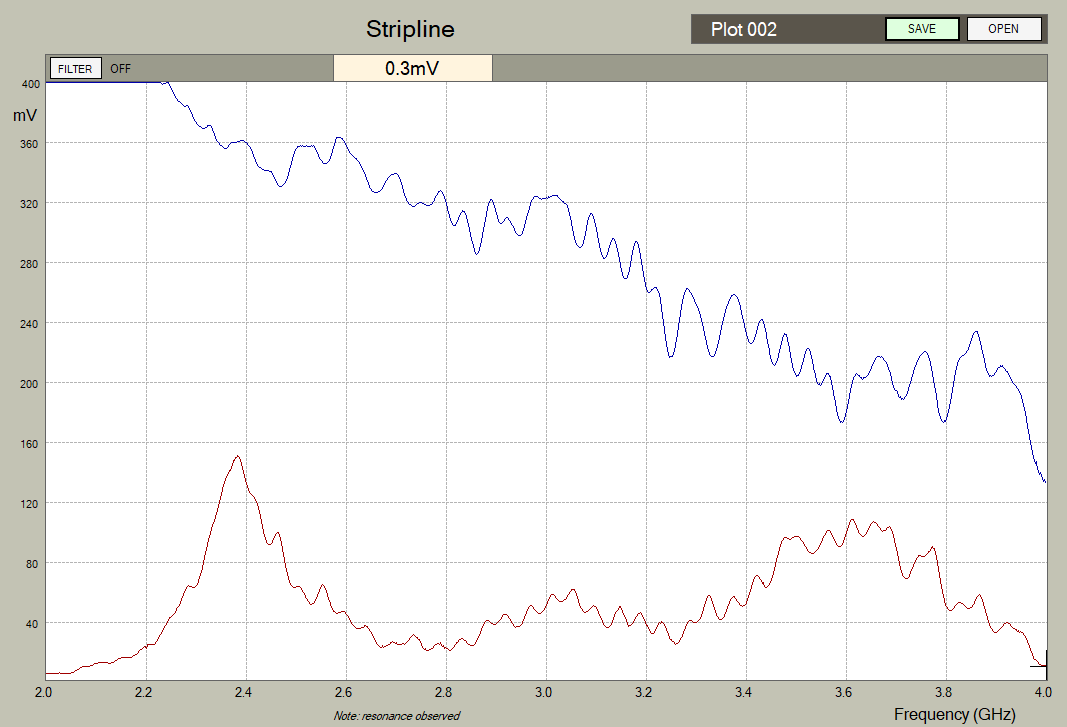
\includegraphics[width=0.8\textwidth]{Plot_2_cropped.png}
    \caption{Graph showing resonance (Red line)}
    \label{fig:freq_responses}
\end{figure}

\section{Analysis of results}

\subsection{Uncertainy and Error Analysis}
The main uncertainty in this experiment came from measuring the distances on the slotted and strip lines
using a ruler with 1mm resolution. This gives the uncertainty of the distance measurements of $\pm0.5$ mm.
The uncertainty in the frequency of the microwave generator in this case is ignored.

The uncertainty in the wavelength and phase velocity is calculated using equations \ref{eq:1} and \ref{eq:2} respectively.
\begin{equation}
    \epsilon_{\lambda} = \frac{2(\epsilon_{P_1}+\epsilon_{Q_1})}{N}
    \label{eq:4}
\end{equation}
\begin{equation}
    \epsilon_{c} = \frac{\epsilon_{\lambda}}{\lambda}\times c
    \label{eq:5}
\end{equation}

The relative uncertainty in S and in the amplitude reflection coefficient can be derived from equations \ref{eq:1} and \ref{eq:2} and shown below.
\begin{equation}
    r_{S} = \frac{1}{2}r_{S^2} = \frac{1}{2} \left[ \frac{\epsilon_{}}{(A+B)^2}+\frac{\epsilon_{}}{(A-B)^2} \right]
    \label{eq:6}
\end{equation}
\begin{equation}
    r_{\rho} = \frac{\epsilon_{S}}{1-S}+\frac{\epsilon_{S}}{1+S}
    \label{eq:7}
\end{equation}

The relative uncertainty in the refractive index of the materials is derived using equation \ref{eq:3} and is shown below.
\begin{equation}
    \epsilon_{n} =\left[ \frac{\epsilon_{d}}{d}+\frac{\epsilon_{R} + \epsilon_{M}}{R-M} \right] \frac{R-M}{d}
    \label{eq:8}
\end{equation}

For the transmission through the resonator the uncertainty was not known as the sweep was performed by the computer. 

All uncertainties are shown in the results tables

\subsection{Wavelength and Phase Velocity}
The expected trend of wavelengths decreasing as the frequency increases is observed in Table \ref{tab:1}.
The phase velocities are close to the expected value $c = 299.8$ mm/ns, however only one result is within the bounds of the uncertainty at 3.6 GHz.
This implies there are some errors in the experiment which are not accounted for in the uncertainty analysis.
One possible cause for this error is that the uncertainty of the distance of minima is far greater than accounted for.
This could be due to the method of finding the points of minima by trial and error.
Another possible cause is the uncertainty in frequency of the microwave generator which may be subject to instrumental drift and is not accounted for in the uncertainty analysis.

\subsection{Amplitude Reflection Coefficient}
The open plug causes a reflection of the wave that is in phase with the incident wave which forms a new wave
shifted a distance $\Delta = \frac{\lambda}{4}$. This is because nodes in the wave superimposed with the anti-phase wave from the short circuit plug.
now become anti-nodes in the new wave and vice versa. It can be seen from Table \ref{tab:2} that the shifted distance is close to the expected value of $\frac{\lambda}{4}$
but still lies out of the range of uncertainties. This again implies errors in the experiment that are not accounted for in the uncertainty analysis.
Beyond aforementioned reasons, this could be due to the fact that the open plug provided some resistance to the wave and so the wave was not perfectly in phase with the incident wave in this case.

The amplitude reflection coefficient is found and is a reasonable value of 0.568 as shown in Table \ref{tab:3}.
This means that the amplitude of the reflected wave is 56.8\% of the amplitude of the incident wave.

\subsection{Velocity of Microwaves in Different Materials}
The refracive indicies of the materials along with their uncertainties are calculated and shown in Table \ref{tab:4}.
From this table, it can be seen that the refractive index of glass is the highest and that of Teflon is the lowest.
This order of refractive indicies for microwaves matches that expected from the materials refractive indicies for visible light mentioned earlier.
Direct comparison of the refractive indicies of the materials for microwaves and visible light is not possible as the refracive indicies vary with wavelength.
However the results are very inconsistent with readings falling well outside the bounds of the uncertainty. This is again
due to errors in the experiment that are not accounted for in the uncertainty analysis.
Another possible cause for this error is that the screw was tightened too much and caused the material to flex producing an 
uneven gap of air between the line and the material.

\subsection{Transmission through a Resonator}
In the initial sweep shown in Fig. \ref{fig:freq_responses} shows no resonance which is expected.
The second sweep shows a peak at 2.38 GHz which is the resonant frequency of the strip line.
This corresponds to a wavelength of 126 mm which is quite close to the distance between the screws, 120mm.
However, the screws may not have been exactly 120 mm apart and so resonant frequency may be off by a small amount.
There could also again be uncertainty in the frequency of the microwave generator due to instrumental drift.

\section{Conclusion}

The phase velocity of microwaves was determined experimentally by investigating standing waves and was found to be within ~1\% of the expected value.
Only one result however was within the bounds of the uncertainty suggesting errors in the setup and method used.
By swapping the open plug for a short circuit plug, the wave shifted by a distance within 5\% of the expected $\frac{\lambda}{4}$.
The amplitude reflection coefficient of brass screws was found to be 0.568 with an small uncertainty of 2\%.
The refractive indicies of glass, Teflon and brass were found for a range of material lengths.
However these values varied widely and were not within the bounds of the uncertainty for the same materials inferring
errors in the setup used. One theory of this was that the screws were tightened too much and caused the material to flex which
produced an uneven gap of air between the line and the material.
Finally, a resonant frequency was found at 2.38 GHz for a 120mm strip line by sweeping the frequency of the microwave generator.
This corresponds to a wavelength 5\% greater than the distance between the screws which could be due to instrumental drift of the microwave generator.

\end{document}